% --- Theoretical Foundations ---
\begin{frame}{Why Does SSL Work?}
  \begin{itemize}\itemsep0.28em
    \item Exploits \textbf{structure} in natural data (spatial context, temporal continuity, language statistics).
    \item Contrastive methods stress \textbf{invariances} to augmentations; reconstruction methods force \textbf{complete} explanations of the input; JEPA emphasizes \textbf{predictive} structure in \textbf{representation space}.
    \item Strong \textbf{linear / low-data probes} suggest encoders expose semantically useful axes for downstream tasks.
    \item Active research: theoretical limits, failure modes (shortcuts), and unified views across the three families above.
  \end{itemize}
\end{frame}

% --- Background: Masked Autoencoders (MAE) ---
% Students skipped the Autoencoders lecture; this grounds the "generative / reconstruction"
% family that JEPA is contrasted against throughout this lecture.
\begin{frame}{Background: Masked Autoencoders (MAE)}
  \begin{itemize}\itemsep0.25em
    \item \textbf{MAE} (He et al., 2022): mask a large fraction ($\sim$75\%) of image patches; the encoder sees \textbf{only visible patches}; a lightweight decoder reconstructs the \textbf{pixels} of the masked ones.
    \item Loss: mean squared error \textbf{in pixel space}, computed on masked patches only.
    \item Asymmetric design (big encoder, small decoder) makes pre-training cheap and scalable.
  \end{itemize}
  \vspace{0.3em}
  \centering
  \begin{tikzpicture}[node distance=0.55cm, every node/.style={font=\scriptsize}]
    \node[draw, rounded corners, fill=blue!10, minimum height=0.9cm, align=center] (input) {Image\\(25\% visible patches)};
    \node[draw, rounded corners, fill=orange!15, minimum height=0.9cm, align=center, right=of input] (enc) {Encoder (ViT)\\visible patches only};
    \node[draw, rounded corners, fill=gray!15, minimum height=0.9cm, align=center, right=of enc] (mask) {+ mask\\tokens};
    \node[draw, rounded corners, fill=orange!15, minimum height=0.9cm, align=center, right=of mask] (dec) {Decoder\\(lightweight)};
    \node[draw, rounded corners, fill=blue!10, minimum height=0.9cm, align=center, right=of dec] (out) {Reconstructed\\pixels};
    \draw[-{Stealth}] (input) -- (enc);
    \draw[-{Stealth}] (enc) -- (mask);
    \draw[-{Stealth}] (mask) -- (dec);
    \draw[-{Stealth}] (dec) -- (out);
    \node[below=0.25cm of out, align=center, text=red!70!black] (loss) {MSE loss on\\masked patches};
    \draw[-{Stealth}, red!70!black, dashed] (out) -- (loss);
  \end{tikzpicture}
  \vspace{0.3em}
  \begin{itemize}\itemsep0.25em
    \item \textbf{Limitation:} the model must explain \emph{every} pixel, including unpredictable texture and noise. JEPA treats this as wasted capacity.
  \end{itemize}
\end{frame}

% --- I-JEPA: Three SSL paradigms (Meta blog) ---
\begin{frame}{SSL Paradigms: Invariant, Generative, and Predictive (JEPA)}
    \begin{itemize}\footnotesize
      \item \textbf{(a) Joint-embedding (invariance):} map views $x,y$ to embeddings and pull compatible pairs together; can bias toward invariance shortcuts.
      \item \textbf{(b) Generative:} decode $\hat{y}$ from context $x$ (and latent $z$), with the loss in \textbf{pixel/input space}; must explain unpredictable detail.
      \item \textbf{(c) JEPA:} predict the \textbf{embedding} $\hat{s}_y$ of $y$ from context and compare to $s_y$ from a target encoder; semantic targets discard irrelevant variability.
    \end{itemize}
    \centering
    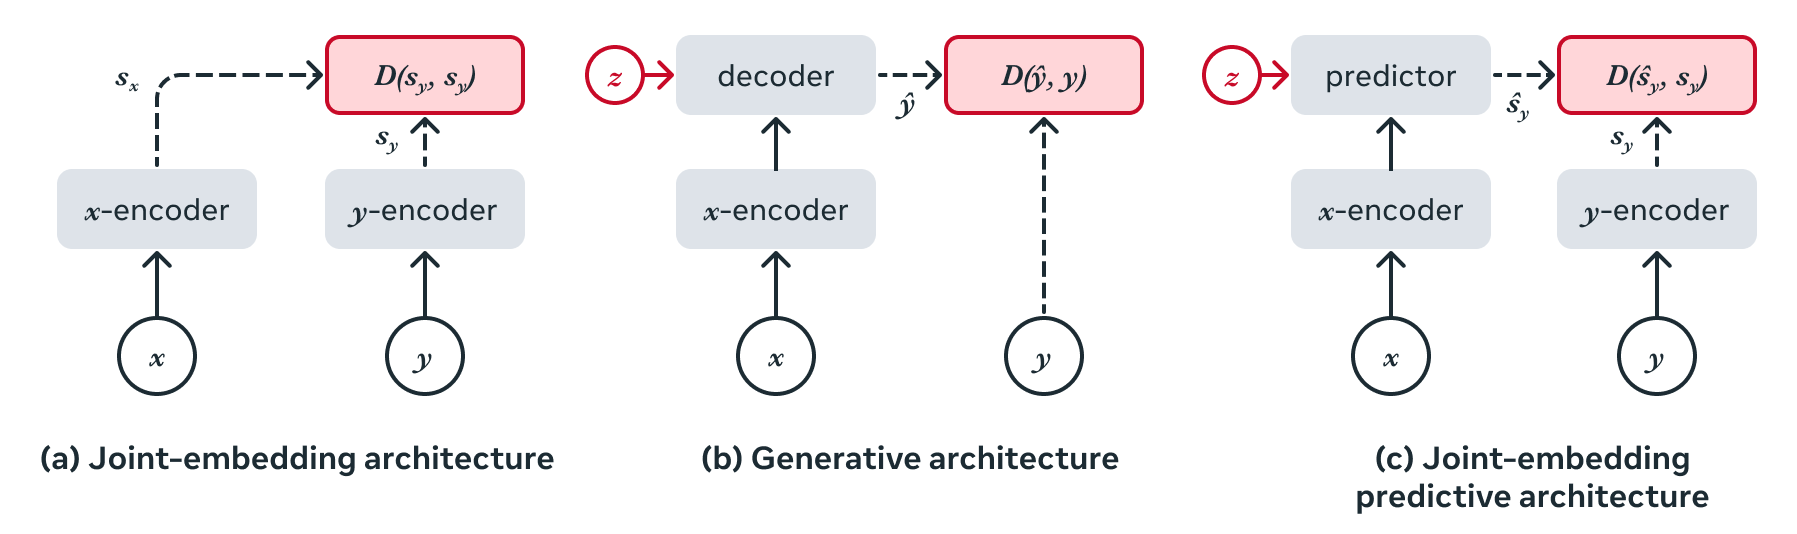
\includegraphics[width=0.8\linewidth, height=0.6\textheight, keepaspectratio]{images/jepa/ijepa_blog_ssl_paradigms.png}
    \linebreak
    {\scriptsize Reference: Adapted from Meta I-JEPA blog.}
\end{frame}

% --- The collapse problem and how JEPA avoids it ---
\begin{frame}{The Collapse Problem and How JEPA Avoids It}
  \begin{itemize}\itemsep0.25em
    \item \textbf{Representation collapse:} if both encoders output a \emph{constant} vector for every input, any similarity or prediction loss is minimized without learning anything.
    \item Three families of \textbf{anti-collapse mechanisms} (Lecture on Contrastive Methods):
    \begin{itemize}\itemsep0.15em
      \item \textbf{Contrastive negatives:} push non-matching pairs apart (SimCLR, MoCo).
      \item \textbf{Information regularization:} keep per-dimension \textbf{variance} up and \textbf{covariance} down (VICReg, Barlow Twins).
      \item \textbf{Architectural asymmetry:} \textbf{stop-gradient} on the target branch + \textbf{EMA teacher} (BYOL, DINO, iBOT); BYOL adds a student-side \textbf{predictor}, DINO \textbf{centers and sharpens} teacher outputs.
    \end{itemize}
    \item \textbf{JEPA inherits the third recipe:} the target encoder is an EMA copy (no gradients flow through targets), and the narrow predictor breaks the symmetry between branches.
    \item Contrastive and non-contrastive objectives are closely related in theory (Garrido et al., 2023), but a full account of \emph{why} EMA plus asymmetry suffices remains an open question.
  \end{itemize}
\end{frame}
